\section{Разработка инструмента генерации программ}
Сравнительный анализ существующих решений для генерации программ показал, что
инструменты, используемые на практике, не подходят для учебных целей. Эти инструменты
в основном заточены под конкретный язык программирования, у многих слабая кастомизация
и нет удобного способа описания шаблона программы. Поэтому было принято решение
разработать собственную систему генерации программ для учебных задач.

\subsection{Требования к системе генерации}
Разрабатываемый инструмент должен обладать следующими возможностями:
\begin{itemize}
    \item Возможность генерации базовых элементов языка программирования;
    \item Поддержка генерации кода на разных языках, чтобы иметь возможность использовать данный
          инструмент в разных обучающих курсах;
    \item Расширяемость, что включает в себя:
          \begin{itemize}
              \item Гибкую систему создания шаблонов для генерации задач;
              \item Возможность настройки параметров генерации;
              \item Высокую вариативность задач, поддержку рандомизации отдельных элементов кода
          \end{itemize}
\end{itemize}

\subsection{Схема генерации программ}
На схеме \ref{generation-steps} предоставлена схема генерации кода программы.
\begin{figure}[ht]
    \begin{center}
        \scalebox{0.8}{
            \includesvg[inkscapelatex=false]{images/generation-steps.svg}
        }
        \caption{\label{generation-steps} Схема генерации кода программы}
    \end{center}
\end{figure}
\clearpage

Разберём ее подробнее. На первом шаге выбирается шаблон, из которого будет генерироваться
программа. Подробнее о шаблонах можно прочитать в разделе \ref{templates}, на текущем этапе нам достаточно
знать, что шаблон --- это некая структура, в которую можно подставить начальное значение для
генератора псевдослучайных чисел (\texttt{seed}) и словарь атрибутов, и получить промежуточное
представление, о котором речь пойдет ниже. \texttt{seed} представляет собой целое
64-битное число, словарь атрибутов сопоставляет строковому ключу список строковых значений,
некоторые из которых могут быть преобразованы в числа

Промежуточное представление является по сути расширением абстрактного синтаксического
дерева (AST)

<<Дерево абстрактного синтаксиса (ДАС) — в информатике конечное помеченное ориентированное дерево, в котором внутренние вершины сопоставлены (помечены) с операторами языка программирования, а листья — с соответствующими операндами. Таким образом, листья являются пустыми операторами и представляют только переменные и константы.>> \cite{ast}

В отличие от чистого AST промежуточное представление, используемое в проекте, хранит
некоторую информацию о синтаксисе языка (или группы языков), в которые оно в дальнейшем
будет интерпретировано. К примеру, в данном дереве могут содержаться скобки в арифметических выражениях,
также промежуточное представление хранит метку (тэг), соответствующую группе языков.

На последнем этапе происходит преобразование промежуточного представления в код. Во время преобразования
элементам промежуточного предоставление сопоставляются элементы синтаксиса конкретного языка программирования.

\subsection{Шаблоны программ}
\label{templates}

\subsubsection{Общие единицы кода для разных языков}
При генерации кода на разных языках можно выделить конструкции, которые имеют схожую
семантику в разных языках, но, при этом, могут отличаться синтаксически. Такими
конструкциями являются к примеру:

\begin{itemize}
    \item Арифметические выражения
    \item Условные ветвления (\texttt{if...else})
    \item Множественный выбор/сопоставление с образцом (\texttt{switch...case, match, when, case...of})
    \item Циклы (\texttt{for, while})
    \item Объявление и инициализация переменных
    \item Объявление, определение и вызов функций
    \item Блоки кода
    \item Инструкции подключения модулей/библиотек (\texttt{import, include})
    \item Строковые и числовые литералы
    \item Объявление классов и структур
    \item \dots
\end{itemize}
\label{syntax-items}

Для каждой из этих конструкций будет достаточно одной сущности в шаблоне, которую смогут образовать
преобразователи промежуточного предоставления для каждого конкретного языка.
\subsubsection{DSL}

Для создания шаблонов программ в дипломном проекте используется язык программирования Kotlin \cite{kotlin}, а
конкретно одна из особенностей языка под названием Kotlin DSL \cite{kotlin-dsl}.

<<Предметно-ориентированный язык (англ. domain-specific language, DSL — «язык, специфический для предметной области») — компьютерный язык, специализированный для конкретной области применения (в противоположность языку общего назначения, применимому к широкому спектру областей и не учитывающему особенности конкретных сфер знаний)>>.
\cite{dsl}

Используемый в проекте DSL является внутренним, то есть написан на языке общего назначения
(в данном случае Kotlin) и имеет точно такой же синтаксис.
\textit{TODO(пример DSL)}

Благодаря возможностям Kotlin DSL, можно воспроизводить в шаблоне древовидную структуру, где параметры
функции --- это параметры в вершине AST, а последний аргумент (ламбда-функция, переданная за пределами скобок)
описывает поддерево.

\subsubsection{Шаблон AST}
Во время выполнения DSL преобразуется в <<шаблон AST>> --- древовидную структуру данных, которая похожа
на AST. В ней могут присутствовать специальные вершины, обозначающие случайное значение или значение
какого-либо атрибута.
При подстановке в нее \texttt{seed} и \texttt{attributes} она преобразуется в промежуточное представление.

\textit{(TODO: добавить шаблонное дерево задачи из предыдущего пункта)}
\subsection{Примеры задач}
\textit{(TODO: добавить примеры задач)}
\subsection{Архитектура системы}
Для поддержки одновременной работы с несколькими пользователями и возможности
добавления шаблонов и валидации ответов студентов разработанная система имеет
клиент-серверную архитектуру с отдельными микросервисами для
некоторых компонент. Благодаря этому удалось добиться конфиденциальности правильных
ответов и контроля над управлением шаблонов.

Клиентская часть представляет собой веб-сайт с помощью которого пользователь может делать
запросы на получение текста или картинки кода по шаблону (задаче). Также имеется возможность
делать запросы напрямую к API в формате JSON \cite{json}.

Серверная часть состоит из нескольких компонент: непосредственно веб-сервер, система генерации
кода и система проверки ответов студентов. В отдельный микросервис выделена система хранения
текстов и изображений программ, состоящая из базы данных, находящейся в изолированном окружении.

Схема архитектуры показана на изображении \ref{architecture}, ниже подробнее описаны отдельные
компоненты.

\begin{figure}[ht]
    \begin{center}
        \scalebox{0.6}{
            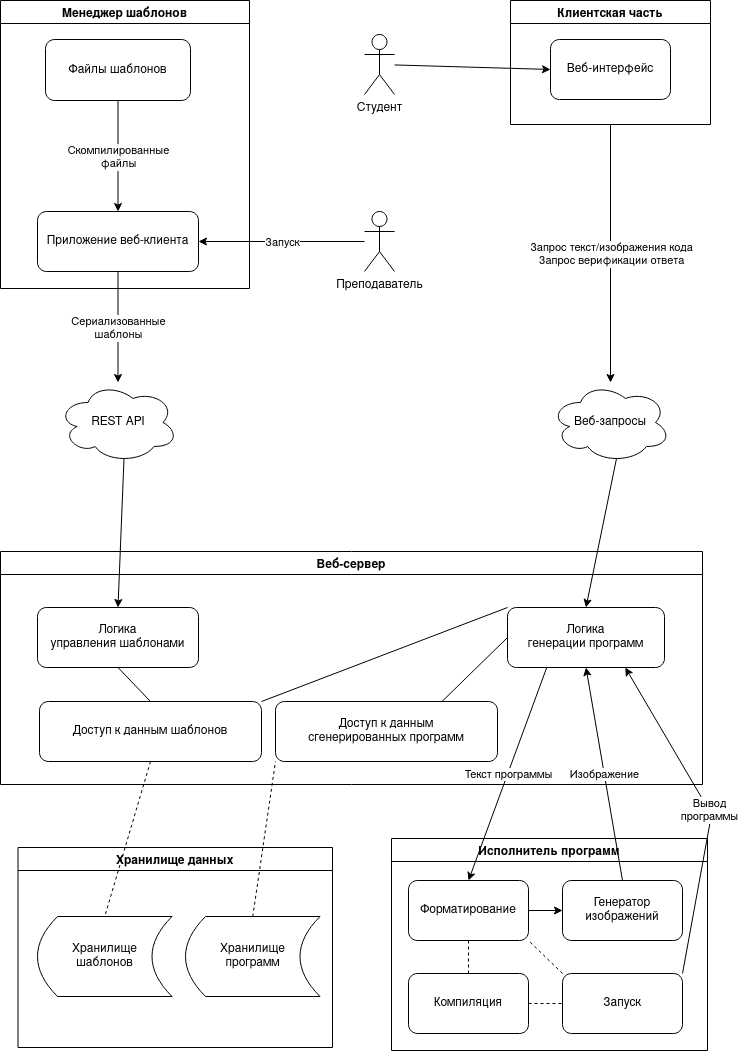
\includegraphics{images/architecture.drawio.png}
            % \includesvg[inkscapelatex=false]{images/architecture.drawio.svg}
        }
        \caption{\label{architecture} Архитектура системы генерации программ}
    \end{center}
\end{figure}
\clearpage

\subsection{Компоненты системы}

\subsubsection{Веб-сервер}
Веб-сервер разделен на две логические части ---
управление шаблонами, доступная только преподавателям
или администраторам, и генерация программ. Первая отвечает
за добавление и удаление шаблонов программ, вторая --- за создание и получение изображения
и текста программы, а так же за верификацию ответов на задачу.

\subsubsection{Исполнитель программ}
Исполнитель программ отвечает за обработку сгенерированного
кода. Он содержит в себе инструмент форматирования кода, инструмент генерации изображения
кода, а также окружение (компилятор и/или интерпретатор), необходимое для выполнения
программы. С помощью данного компонента осуществляется генерация изображения и получение
вывода программы при ее запуске.

Исполнитель вынесен в отдельный компонент так как ему необходимо специальное окружение
(установленные компиляторы, интерпретаторы, средства форматирования).

\subsubsection{База данных}
\label{db-model}
Для поддержки работы с несколькими пользователями необходимо хранить шаблоны и данные о
сгенерированных программах в базе данных.

В базе сгенерированных программ хранятся параметры генерации,
которые, вместе с
идентификатором задачи, выступают ключом. Также в ней хранятся текст программы,
изображение и вывод программы при запуске.

\label{template-db} В базе шаблонов хранятся шаблоны программ, тэг, соответствущий языку или группе
языков, для которых написан этот шаблон, и имя шаблона (задачи), которое является ключом.

\subsubsection{Сторона клиента}
На клиентской стороне пользователь может как взаимодействовать напрямую с сервером,
делая запросы через строку браузера и получая ответ в формате HTML, так и через
специальные образовательные платформы по типу Moodle \cite*{moodle}.

\subsubsection{Менеджер шаблонов}
Для создания и управления шаблонами программ на стороне клиента используется отельная
программа --- менеджер шаблонов (Template Manager на схеме). С помощью нее при добавлении текст шаблона
преобразуется в машиночитаемый вид \textit{(TODO: вставить ссылку на детали реализации)}
и затем, вместе с прочей необходимой информацией (названием, тэгом) отправляется на сервер
для сохранения в базу шаблонов (см. \ref{template-db}).
